\documentclass{beamer}

\usepackage{metalogo}
\title{Introduction to \XeLaTeX}
\author{Stefano Coretta}
\date{February 4, 2016}

\usetheme{Szeged}
\usecolortheme{beaver}

\usepackage{amsmath}

\usepackage{polyglossia}
	\setmainlanguage{english}
\usepackage{fontspec}
	\defaultfontfeatures{Mapping=tex-text}
	\setmainfont{FreeSans}
	\setsansfont{FreeSans}
	\setmonofont{FreeMono}
	\setromanfont[Renderer=ICU]{Charis SIL}

\usepackage{ctable,multicol,multirow,array,listings}
	\lstset{frame = single,
	   numbers = left,
	   breaklines = true,
	   breakindent = 0pt,
	   basicstyle=\ttfamily}
\usepackage{graphicx}
    \graphicspath{{./img/}}
\usepackage{color}

\usepackage{etoolbox}

\setbeamertemplate{caption}[numbered]
\setbeamertemplate{section in toc}[sections numbered]
\setbeamertemplate{subsection in toc}[subsections numbered]
\setbeamertemplate{footline}
{%
  \begin{beamercolorbox}[colsep=1.5pt]{upper separation line foot}
  \end{beamercolorbox}
  \hbox{%
    \begin{beamercolorbox}[wd=0.333333\paperwidth, ht=2.5ex, dp=1.125ex, center]{title in head/foot}%
      \usebeamerfont{author in head/foot}\insertshortauthor
    \end{beamercolorbox}%
    \begin{beamercolorbox}[wd=0.333333\paperwidth, ht=2.5ex, dp=1.125ex, center]{title in head/foot}%
      \usebeamerfont{title in head/foot}\insertshorttitle
    \end{beamercolorbox}%
    \begin{beamercolorbox}[wd=0.333333\paperwidth, ht=2.5ex, dp=1.125ex, center]{title in head/foot}%
      \usebeamerfont{title in head/foot}\insertframenumber/\inserttotalframenumber\hspace*{2ex}
    \end{beamercolorbox}}
  \begin{beamercolorbox}[colsep=1.5pt]{lower separation line foot}
  \end{beamercolorbox}
}

\DeclareRobustCommand{\BibTeX}{%
  {\normalfont B\kern-.05em{\scshape i\kern-.025em b}\kern-.08em \TeX}%
}

%%%%%%%%%%%%%
%%% DOCUMENT %%%
%%%%%%%%%%%%%


\begin{document}

%%%%%%%%%%%%%%%%%%%%%%%%%%%%%%%%%%%

\begin{frame}
	\maketitle
\end{frame}

%%%%%%%%%%%%%%%%%%%%%%%%%%%%%%%%%%%

%\begin{frame}
%	\frametitle{Contents}
%	\tableofcontents
%\end{frame}

%%%%%%%%%%%%%%%%%%%%%%%%%%%%%%%%%%%

\section{Introduction}

%%%%%%%%%%%%%%%%%%%%%%%%%%%%%%%%%%%

\begin{frame}
	\frametitle{What is \XeLaTeX{}?}
	
\begin{itemize}
\item it is a mark-up language for typesetting and text writing (and more)
\item it is a variant of the \LaTeX{} format that introduced full Unicode support and \texttt{.ttf}, \texttt{.otf} font handling
\item it is implemented by the \XeTeX{} engine, that is derived from the \TeX{} system
\end{itemize}

\end{frame}

%%%%%%%%%%%%%%%%%%%%%%%%%%%%%%%%%%%

\begin{frame}
	\frametitle{How does it work?}
	
\begin{itemize}
\item put the \XeLaTeX{} code in a \texttt{.tex} with the content of your document
\item the \XeTeX{} engine reads and typeset the code
\item a \texttt{.pdf} file with your document is produced
\end{itemize}

\end{frame}

%%%%%%%%%%%%%%%%%%%%%%%%%%%%%%%%%%%

\begin{frame}
	\frametitle{Get it!}
	
\begin{itemize}
%\item download a \TeX{} distribution (\textit{distro})
%\begin{itemize}
%\item MikTeX
%\item TeXlive 
%\item MacTeX
%\end{itemize}
\item a \textit{distro} contains both the systems and the engines, plus software that ease the typesetting process
\item \textbf{any problems or questions?}
\end{itemize}

\end{frame}

%%%%%%%%%%%%%%%%%%%%%%%%%%%%%%%%%%%

\section{Typeset}
\subsection{First steps}

%%%%%%%%%%%%%%%%%%%%%%%%%%%%%%%%%%%

\begin{frame}[fragile]
	\frametitle{Document class}
	
\begin{lstlisting}
\documentclass{article}

\begin{document}

Hello, World!

\end{document}
\end{lstlisting}

\end{frame}

%%%%%%%%%%%%%%%%%%%%%%%%%%%%%%%%%%%

\begin{frame}[fragile]
	\frametitle{Title}
	
\begin{lstlisting}
\documentclass{article}

\title{Introduction to science}
\author{John Smith}
\date{}

\begin{document}
\maketitle

Hello, World!

\end{document}

\end{lstlisting}

\end{frame}

%%%%%%%%%%%%%%%%%%%%%%%%%%%%%%%%%%%

\begin{frame}[fragile]
	\frametitle{Headings}
\footnotesize
\begin{lstlisting}
\documentclass[12pt,a4paper]{article}

\title{Introduction to science}
\author{John Smith}
\date{}

\begin{document}
\maketitle
\tableofcontents

\section{Introduction}
Hello, World!

\subsection{Background}
Text...

\end{document}
\end{lstlisting}

\end{frame}

%%%%%%%%%%%%%%%%%%%%%%%%%%%%%%%%%%%

\subsection{Packages and format}

%%%%%%%%%%%%%%%%%%%%%%%%%%%%%%%%%%%

\begin{frame}[fragile]
	\frametitle{Packages}
	
Put the following code in the \textbf{preamble} (just after \verb+\documentclass+):


\begin{lstlisting}
\usepackage{fontspec}
  \setmainfont{Times New Roman}
\usepackage{polyglossia}
  \setmainlanguage{english}
\end{lstlisting}

\end{frame}

%%%%%%%%%%%%%%%%%%%%%%%%%%%%%%%%%%%

\begin{frame}
	\frametitle{Text layout}
	

For a new paragraph, leave an empty line.

This is the new paragraph.
You can \textit{format} your \textbf{text}.

For a footnote.\footnote{This is a footnote.}

% This is a comment (it will not be typeset)

\end{frame}

%%%%%%%%%%%%%%%%%%%%%%%%%%%%%%%%%%%

\begin{frame}[fragile]
	\frametitle{Text layout}
	
\begin{lstlisting}
For a new paragraph, leave an empty line.

This is the new paragraph.
You can \textit{format} your \textbf{text}.

For a footnote.\footnote{This is a footnote.}

% This is a comment (it will not be typeset)
\end{lstlisting}

\end{frame}

%%%%%%%%%%%%%%%%%%%%%%%%%%%%%%%%%%%

\begin{frame}[fragile]
	\frametitle{Bullet and numbered lists}
\begin{lstlisting}
\begin{itemize}
\item List: one, two
\item another point
\item yet another
\end{itemize}
\end{lstlisting}
\end{frame}

%%%%%%%%%%%%%%%%%%%%%%%%%%%%%%%%%%%

\begin{frame}
	\frametitle{Bullet and numbered lists}
\begin{itemize}
\item List: one, two
\item another point
\item yet another
\end{itemize}
\end{frame}

%%%%%%%%%%%%%%%%%%%%%%%%%%%%%%%%%%%

\begin{frame}[fragile]
	\frametitle{Bullet and numbered lists}
\begin{lstlisting}
\begin{itemize}
\item List: one, two
\item another point
  \begin{enumerate}
  \item three
  \item four
  \end{enumerate}
\end{itemize}
\end{lstlisting}
\end{frame}

%%%%%%%%%%%%%%%%%%%%%%%%%%%%%%%%%%%

\begin{frame}
	\frametitle{Bullet and numbered lists}
\begin{itemize}
\item List: one, two
\item another list
  \begin{enumerate}
  \item three
  \item four
  \end{enumerate}
\end{itemize}
\end{frame}

%%%%%%%%%%%%%%%%%%%%%%%%%%%%%%%%%%%


\section{Common commands}
\subsection{Standard elements}

%%%%%%%%%%%%%%%%%%%%%%%%%%%%%%%%%%%

\begin{frame}[fragile]
    \frametitle{Figures}
In your preamble put:
\begin{lstlisting}
\usepackage{graphicx}
\end{lstlisting}


In your document environment put:
\begin{lstlisting}
\begin{figure}
\centering
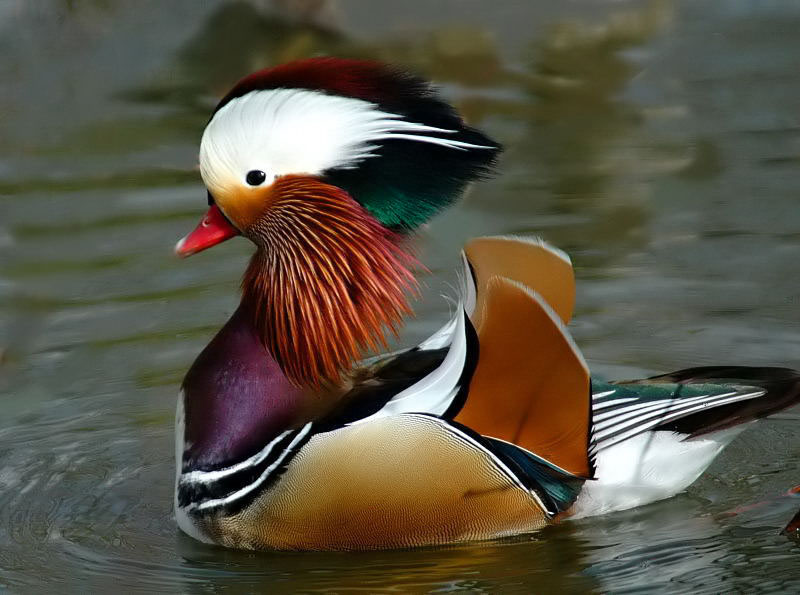
\includegraphics[width=0.6\textwidth]{mandarin_duck}
\caption{Mandarin duck.}  
\end{figure}
\end{lstlisting}

\end{frame}

%%%%%%%%%%%%%%%%%%%%%%%%%%%%%%%%%%%

\begin{frame}
    \frametitle{Figures}

\begin{figure}
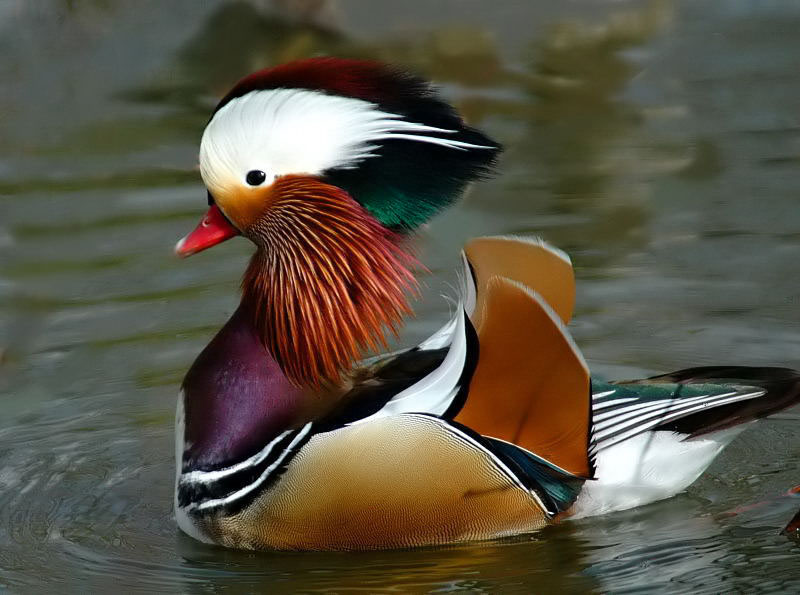
\includegraphics[width=0.6\textwidth]{mandarin_duck}
\caption{Mandarin duck.}  
\end{figure}

\end{frame}

%%%%%%%%%%%%%%%%%%%%%%%%%%%%%%%%%%%

\begin{frame}[fragile]
	\frametitle{Tables}

In your preamble, load \texttt{ctable}:
\begin{lstlisting}
\usepackage{ctable}
\end{lstlisting}

In your document, insert:
\begin{lstlisting}
\ctable[caption=Gender distribution,
pos=t
]{lcc}{}{
\FL
 & Male & Female \ML
Young & 85 & 65 \NN
Old & 100 & 147 \LL
}
\end{lstlisting}

\end{frame}

%%%%%%%%%%%%%%%%%%%%%%%%%%%%%%%%%%%

\begin{frame}
	\frametitle{Tables}

\ctable[caption=Genders,
pos=t
]{lcc}{}{
\FL
 & Male & Female \ML
Young & 85 & 65 \NN
Old & 100 & 147 \LL
}

\end{frame}

%%%%%%%%%%%%%%%%%%%%%%%%%%%%%%%%%%%


\begin{frame}[fragile]
	\frametitle{Escape character}
	
Reserved characters must be \textbf{escaped} with the escape characters, which is the backslash \textbackslash.

\vspace{2ex}
\centering
\begin{tabular}{ll}
\verb+\&+ & \& \\ 
\verb+\%+ & \% \\ 
\verb+\#+ & \# \\ 
\verb+\_+ & \_ \\ 
\verb+\textbackslash+ & \textbackslash
\end{tabular} 

\end{frame}

%%%%%%%%%%%%%%%%%%%%%%%%%%%%%%%%%%%

\begin{frame}
    \frametitle{Maths}

The formula can be reduced to $\int_0^\infty \mathrm{e}^{-x}\,\mathrm{d}x$.

\begin{equation}
    \cos (2\theta) = \cos^2 \theta - \sin^2 \theta
\end{equation}

\begin{equation}
    \sqrt[n]{1+x+x^2+x^3+\ldots}
\end{equation}

\begin{equation}
    \sum_{i=1}^{10} t_i
\end{equation}

\end{frame}

%%%%%%%%%%%%%%%%%%%%%%%%%%%%%%%%%%%

\begin{frame}[fragile]
    \frametitle{Maths}

\footnotesize
\begin{lstlisting}
I love Maths! $\int_0^\infty \mathrm{e}^{-x}\,\mathrm{d}x$.

\begin{equation}
    \cos (2\theta) = \cos^2 \theta - \sin^2 \theta
\end{equation}

\begin{equation}
    \sqrt[n]{1+x+x^2+x^3+\ldots}
\end{equation}

\begin{equation}
    \sum_{i=1}^{10} t_i
\end{equation}
\end{lstlisting}

\end{frame}

%%%%%%%%%%%%%%%%%%%%%%%%%%%%%%%%%%%

\subsection{Special functions}

%%%%%%%%%%%%%%%%%%%%%%%%%%%%%%%%%%%

\begin{frame}[fragile]
    \frametitle{Cross-referencing}

\begin{itemize}
\item use \verb+\label{...}+ to index headings, tables, images, etc. Put the lable within \{ \}
\item reference them using \verb+\ref{...}+
\item check the package \texttt{cleveref} for advanced cross-referencing
\end{itemize}

\end{frame}

%%%%%%%%%%%%%%%%%%%%%%%%%%%%%%%%%%%

\begin{frame}[fragile]
	\frametitle{Cross-referencing}
\begin{lstlisting}
\section{Methodology}
\label{sec:method}
You can cross-ref almost anything: headings, figures, tables, equations...

\section{Conclusions}
As I said in section \ref{sec:method}... In equation \ref{fig:duck}...

\end{lstlisting}
\end{frame}

%%%%%%%%%%%%%%%%%%%%%%%%%%%%%%%%%%%

\begin{frame}[fragile]
	\frametitle{Cross-referencing}
\begin{lstlisting}
\begin{figure}
    \includegraphics{image}
    \caption{My fancy image.}
    \label{fig:image}    
\end{figure}

As you can see in Figure \ref{fig:image} [...]

\end{lstlisting}
\end{frame}

%%%%%%%%%%%%%%%%%%%%%%%%%%%%%%%%%%%

\begin{frame}[fragile]
	\frametitle{Cross-referencing}
\begin{lstlisting}
\ctable[caption = My useless table,
label = tab:table
]{cc}{}{
\FL
This is just & a useless table \LL
}

As you can see in Table \ref{tab:table} [...]

\end{lstlisting}
\end{frame}

%%%%%%%%%%%%%%%%%%%%%%%%%%%%%%%%%%%

\iffalse

\begin{frame}
    \frametitle{Bibliography}

\begin{itemize}
    \item automatic handling of bibliography with \BibTeX
    \item you need a \texttt{.bib} file and a \texttt{.bst} file
    \begin{itemize}
        \item the \texttt{.bib} file contains your bibliography entries
        \item the \texttt{.bst} file is the bibliography style file
    \end{itemize}
    \item the \texttt{natbib} package helps you put citations in your document
\end{itemize}

\end{frame}

%%%%%%%%%%%%%%%%%%%%%%%%%%%%%%%%%%%

\begin{frame}[fragile]
	\frametitle{Bibliography}
	
Call the \texttt{natbib} package in the preamble, with the option \texttt{numbers} for IEEE like style:
\begin{lstlisting}
\usepackage[numbers]{natbib}
\end{lstlisting}

Set the bibliography style (\texttt{plainnat}) and \texttt{.bib} file at the end of your document, before \verb+\end{document}+

\begin{lstlisting}
\bibliographystyle{plainnat}
\bibliography{mybib}
\end{lstlisting}


\end{frame}

%%%%%%%%%%%%%%%%%%%%%%%%%%%%%%%%%%%

\begin{frame}[fragile]
	\frametitle{Bibliography}
	
Call the \texttt{natbib} package in the preamble, with the option \texttt{numbers} for Harvard like style:
\begin{lstlisting}
\usepackage{natbib}
\end{lstlisting}

Set the bibliography style (\texttt{agsm}) and \texttt{.bib} file at the end of your document, before \verb+\end{document}+

\begin{lstlisting}
\bibliographystyle{dcu}
\bibliography{mybib}
\end{lstlisting}


\end{frame}

%%%%%%%%%%%%%%%%%%%%%%%%%%%%%%%%%%%

\begin{frame}[fragile]
    \frametitle{Bibliography}

In your document, you can use the \verb+\cite+ commands:

\begin{lstlisting}
According to \citet{darwin1859}, we have a common ancestor with [...]. However, it is more complex \citep{asimov1951}.
\end{lstlisting}

The output depends on the chosen style.

\end{frame}

%%%%%%%%%%%%%%%%%%%%%%%%%%%%%%%%%%%

\begin{frame}
    \frametitle{Bibliography}

\begin{figure}
    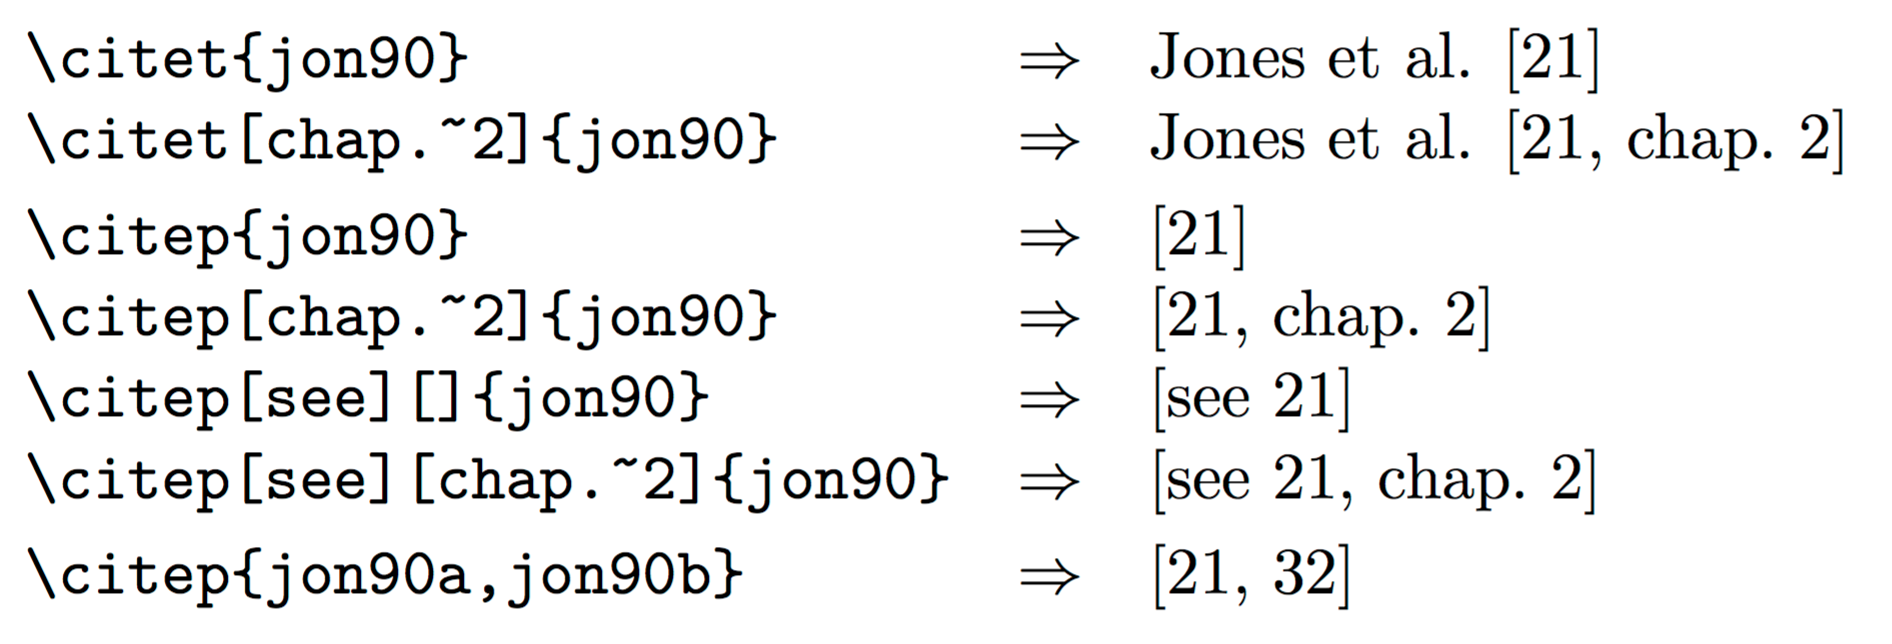
\includegraphics[width=\textwidth]{natbib-num}
\end{figure}


\end{frame}

%%%%%%%%%%%%%%%%%%%%%%%%%%%%%%%%%%%

\begin{frame}
    \frametitle{Bibliography}

\begin{figure}
    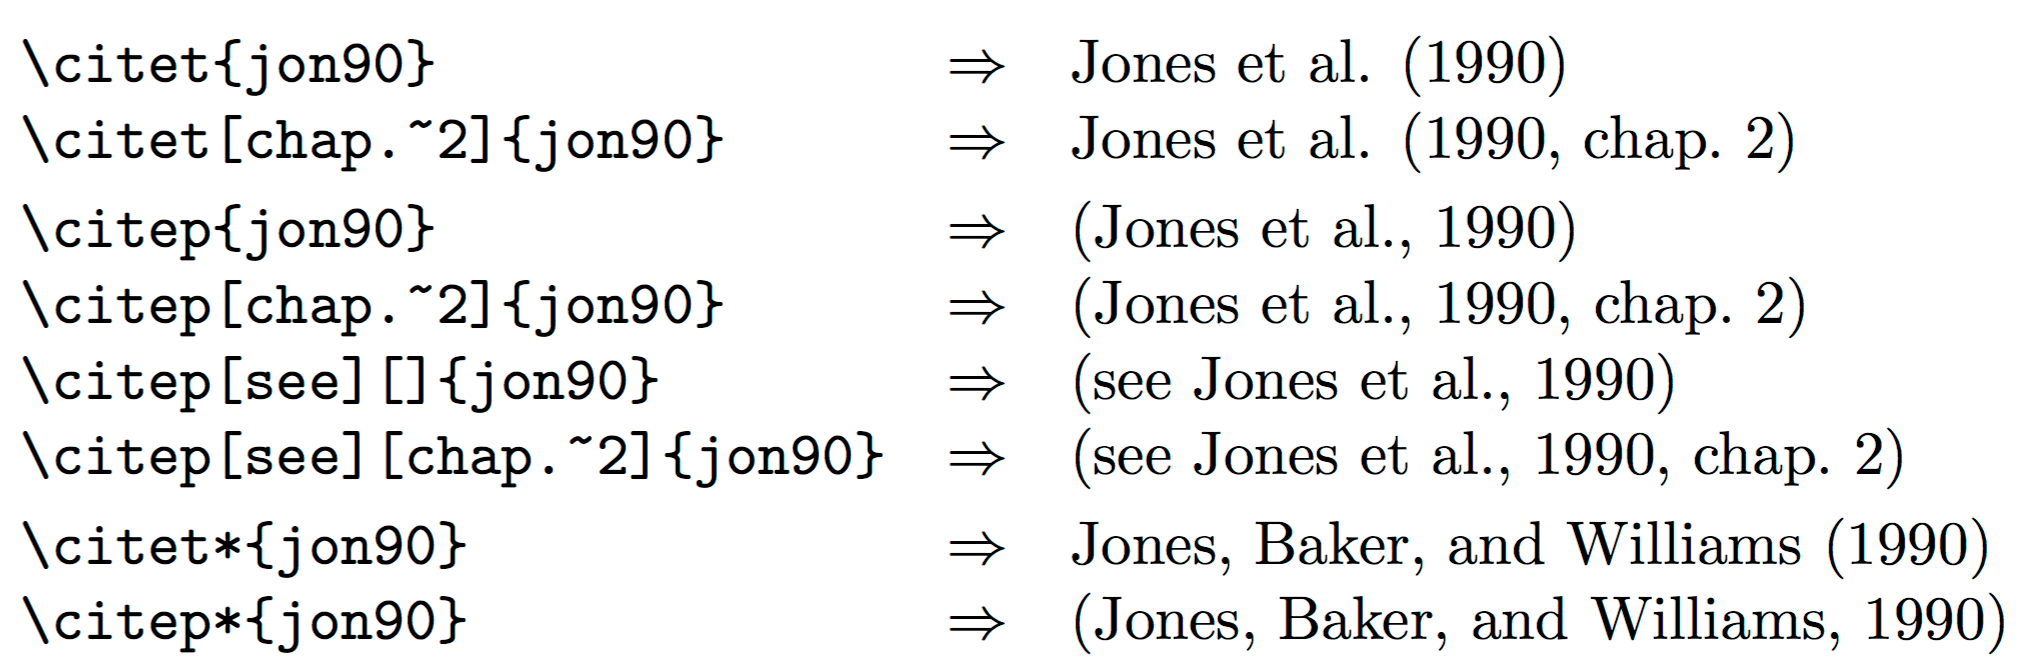
\includegraphics[width=\textwidth]{natbib-ay}
\end{figure}


\end{frame}

\fi
%%%%%%%%%%%%%%%%%%%%%%%%%%%%%%%%%%%

\lstdefinestyle{pythonico}{keywordstyle=\bfseries\color{green!40!black},
  commentstyle=\itshape\color{purple!40!black},
  identifierstyle=\color{blue},
  stringstyle=\color{red},showstringspaces=false,}

\begin{frame}[fragile]
    \frametitle{Code listings}

\begin{lstlisting}[language=Python,style=pythonico]
rangelist = range(10)
print rangelist
[0, 1, 2, 3, 4, 5, 6, 7, 8, 9]
for number in rangelist:
    if number in (3, 4, 7, 9):
        break
    else:
        continue
# Comment
if rangelist[1] == 2:
    print "The second item is 2"
else:
    print "Dunno"
\end{lstlisting}

\end{frame}

%%%%%%%%%%%%%%%%%%%%%%%%%%%%%%%%%%%

\begin{frame}[fragile]
    \frametitle{Code listings}

\begin{lstlisting}
\lstset{keywordstyle=\bfseries\color{green!40!black},commentstyle=\itshape\color{purple!40!black},identifierstyle=\color{blue},stringstyle=\color{red},showstringspaces=false,}

\begin{lslisting}
[your code]    
\end{lslisting}

\lstinputlisting[language=Python]{source_filename.py}

\end{lstlisting}

\end{frame}

%%%%%%%%%%%%%%%%%%%%%%%%%%%%%%%%%%%

\begin{frame}
    \frametitle{Modular documents}
    
\begin{itemize}
    \item file structure of your document
    \item modularity is good for theses/dissertations
    \item Project folder
    \begin{itemize}
        \item \texttt{main.tex}: it's the main document that you compile
        \item \texttt{tex}: is the folder where you put the \texttt{.tex }subfiles
        \item \texttt{img}: is the folder where you put the images
    \end{itemize}
\end{itemize}

\end{frame}

%%%%%%%%%%%%%%%%%%%%%%%%%%%%%%%%%%%

\begin{frame}[fragile]
    \frametitle{Modular documents}
    
\begin{lstlisting}
\documentclass{memoir}

\usepackage{graphicx}
    \graphicspath{{./img/}} % set the folder with images
\usepackage{...} % load your packages as usual

\begin{document}

\chapter{Introduction}
\label{ch:introduction}
\chapter{Methods}
\label{ch:methods}


\end{document}
    
\end{lstlisting}

\end{frame}

%%%%%%%%%%%%%%%%%%%%%%%%%%%%%%%%%%%

\begin{frame}
    \frametitle{Resources}
    
\begin{itemize}
    \item LaTeX Wikibook: \url{https://en.wikibooks.org/wiki/LaTeX}
    \item TeX StackExchange: \url{http://tex.stackexchange.com}
    \item Comprehensive \TeX{} Archive Network (CTAN): \url{http://www.ctan.org}
    \item \texttt{memoir} class: \url{http://www.ctan.org/tex-archive/macros/latex/contrib/memoir/}
    
    \item For stats: Sweave (LaTeX + R) \url{http://www.statistik.lmu.de/~leisch/Sweave/}
    \item versioning system: git + \TeX{} \url{http://stackoverflow.com/a/6190412/2804314}
\end{itemize}

\end{frame}




% TODO stats

\end{document}
